\documentclass{article}
\usepackage{amssymb}
\usepackage[utf8]{inputenc}
\usepackage{amsmath}
\usepackage{listings}
\usepackage{stmaryrd}
\usepackage{graphics,graphicx}
\usepackage[colorinlistoftodos]{todonotes}
\usepackage{import}
\usepackage{mathpartir}
\usepackage{aliascnt}
\usepackage{array}
\usepackage{comment}
\usepackage{indentfirst}
\usepackage{tikz}
\usetikzlibrary{matrix}
\usepackage{subcaption}
\usepackage{tikz}
\usetikzlibrary{calc, shapes, backgrounds}
\usepackage{verbatim}
\usepackage{pgf}
\usepackage{tikz}
\usepackage{tikz-qtree}
\usepackage{pgfplots}
\usepackage{caption,capt-of}
\usepackage{subcaption}
\pgfplotsset{compat=1.10}
\usetikzlibrary{shapes.geometric,arrows,fit,matrix,positioning}
\tikzset
{
    treenode/.style = {circle, draw=black, align=center, minimum size=0.1cm},
    subtree/.style  = {isosceles triangle, draw=black, align=center, minimum height=0.5cm, minimum width=0.5cm, shape border rotate=90, anchor=north}
}
\usetikzlibrary{graphs} % LaTeX
\usetikzlibrary[graphs] % ConTeXt
\usetikzlibrary{arrows,automata}
\usepackage{hyperref}
\lstset{
    language=c,
    numbers=left,
    showstringspaces=false,
    showspaces=false,
    numberstyle=\tiny,
    resetmargins=true,
}

\begin{document}
\begin{comment}
\section{Introduction}

Reasoning on concurrent programs is really hard. One of the fundamental problems is necessity the of doing a set of operations simultaneously or indivisibly for correctness reasons. Partially completed set operations may result in inconsistency in the data structure. However, there are cases in which temporal inconsistency is acceptable, specifically postponing any work that is not immediately necessary. Each process only does what it has to do. With this technique, the multiprocessing capability supplied by processors is utilized. This is particularly advantageous in the case in which work cannot be done immediately, and a process 
would have have to wait; instead, it can relegate the work to another process, to 
be done when feasible[Lehman]. 

The general design for this type of programming pattern is simple and efficient. Simply, no reader locks are used and no lock per node is allowed. Updater processes are mutually exclusive via a writer lock that prevents simultaneous update of a node by more than one process. As a result of this concurrent setting, there is a set of reader processes and a set of updater processes with a processes or set of processes to reclaim memory locations where nodes in the free list reside. An example of delaying of a work occurs in garbage collection. It is generally unnecessary to collect garbage immediately after it is generated.

Instances of this framework are seen intensively in concurrent memory reclamation algorithms like RCU (Read-Copy-Update), Hazard Pointers and Epoch-Based reclamation. Using those programming patterns in non-blocking algorithms are extremely complicated which makes them error-prone in usage. This comes with the need to verify correctness of non-blocking algorithms. The reasoning naturally about interactions between threads in the framework and their instances are so subtle and very challenging [TODO: Is there any proof?]. There is an intensive research effort on formalizing relaxed memory reclamation algorithms and proof methods to reason on the algorithms[AlexeyESOP13]. Using heavy-weight proof methods to check correctness [TODO: What is correctness?] results in complicated proofs.
We propose a light-weight type system, rather than full formal system. It is light but it gives very strong guarantees. 
\end{comment}
\section{Motivating example}

[Might be interesting to consider Red/Black trees in RCU.  The rotations are beyond what we currently support, but should be sound if done in the style of a purely functional datastructure.]
RCU has been used to construct a number of concurrent data structures such as:
\begin{itemize}
\item Concurrent Linked-List
\item Concurrent Hash Tables [Resizable, scalable, concurrent hash tables via relativistic programming]
\item Concurrent Red-Black trees [Relativistic red-black trees]
\item Software Transactional Memory implementations
\end{itemize}
Enforcing readers to see the modifications in a particular order, linearizability,  in red-black trees and hash tables in such optimistic concurrent setting as a correctness criteria is very important. 
\subsection{Informal Reasoning on Linked List}
\begin{table}[]
	\begin{tabular}{|p{7cm}|p{7cm}|}
		Read & Update \\
		
\begin{lstlisting}
struct node_p{
  void* data;
  node_p next;
}		
node_p<rcu> head;
	
data Read(data toRead){
  data result;	
  rcuRead{
    node_p<rcuIterator> itr; 
    itr=head;     
    while(itr != NULLl){
      if(itr.data == toRead)
	    break;
	  itr= itr.next;
    }
    result = itr.data;
  }
  return result;
}
		\end{lstlisting} &
		
		\begin{lstlisting}
void Update(data toDel){

 rcuMutate{
   node_p <rcuIterator>itr;
   node_p<rcuIterator> prev;

   itr=prev=head;    
   if(itr != NULL){
    while(itr != NULL){
     if(itr.data == toDel)
       break;
     prev = itr;
     itr = itr.next;
    }
   }
   prev.next = itr.next;    
   }		
   asyncDelayedFree(free,itr);			
}
		\end{lstlisting} 
	\end{tabular}
	
	\caption{RCU-Linked-List Implementation.}
	\label{tab:rculist}
\end{table}

In RCU based non-blocking linked list implementation, generally the implementation pattern looks similar to the one shown in Table ~\ref{tab:rculist}. However, the implementation shown in Table ~\ref{tab:rculist} includes types parameterized under our type system rules.
\paragraph{Update}  : \textsf{rcuMutate} block in between lines (3-17) is defined as  a mutual exclusive scope where only one mutator thread can be inside. 

\textsf{asyncDelayedFree} at line 18 is not inside \textsf{rcuMutate}. In other words, asynchronous memory reclamation call is not handled inside a mutually exclusive block.  [TODO: Showing that atomic\{traverse;unlink;reclaim\} == rcuMutate\{traverse;unlink\} asyncDelayedFree]. See \textbf{mutator axioms} in section  ~\ref{mutatoraxioms}.

\paragraph{Read} : \textsf{rcuRead} block in between lines (9-18) is defined as a read only scope in which only reader threads can have access. Many reader threads can have access to this block simultaneously even though threre exists an iterator pointer from the mutator thread at the same time.  Pictorially, the interleaving of reader and writer threads are shown as in the following Figure ~\ref{fig:readlist} , Figure ~\ref{fig:mutatelist} and Figure ~\ref{fig:unlinkedlist} : 

\begin{figure}
\centering
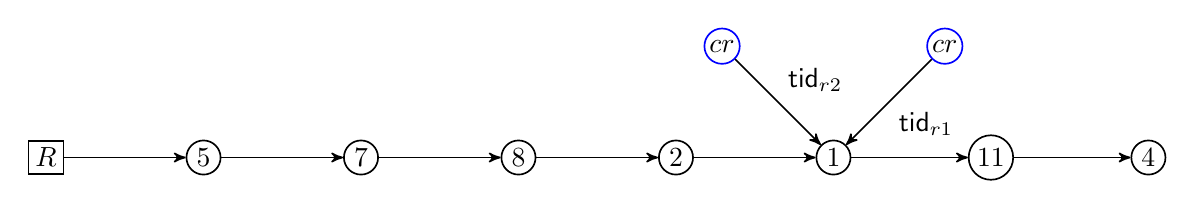
\begin{tikzpicture}[>=stealth',node distance=2cm,semithick,auto]
\tikzstyle{hollow node}=[circle,draw,inner sep=1.5]
\tikzstyle{sub node}=[triangle,draw,inner sep=1.5]
\tikzstyle{solid node}=[rectangle,draw,inner sep=2.5]

\tikzset{
	red node/.style={rectangle,draw=red,fill=red,inner sep=2.2},
	blue node/.style={rectangle,draw=blue,inner sep=2.5},
	reader node/.style={circle,draw=blue,inner sep=1},
	writer node/.style={circle,draw=green,inner sep=1}
}
 
    \node[solid node] (R) {$R$};
    \node[hollow node] (5) [right of=R] {$5$};
    \node[hollow node] (7) [right of=5] {$7$};
   \node[hollow node] (8) [right of=7] {$8$};
    \node[hollow node] (2) [right of=8] {$2$};
    \node[hollow node] (1) [right of=2] {$1$};
    \node[hollow node] (11) [right of=1] {$11$};
    \node[hollow node] (4) [right of=11] {$4$};
  \node[reader node] (r1) [above right of= 1]  {$cr$};
    \node[reader node] (r2)  [above left of= 1] {$cr$};

    \path[->]   (R) edge node {} (5)
                (5) edge node {} (7)
		(7) edge node {} (8)
		(8) edge node {} (2)
		(2) edge node {} (1)
		(1) edge node {} (11)
		(11) edge node {} (4)                
		(r1) edge node {$\textsf{tid}_{r1}$} (1)
		(r2) edge node {$\textsf{tid}_{r2}$} (1)
;
\end{tikzpicture}
\caption{Two concurrent reader threads with $\textsf{tid}_{r1}$ and $\textsf{tid}_{r2}$ ids are on the node with value 1. These threads have their own iterators $\textsf{cr}$ on linked list. }
\label{fig:readlist}
\end{figure}

\begin{figure}
\centering
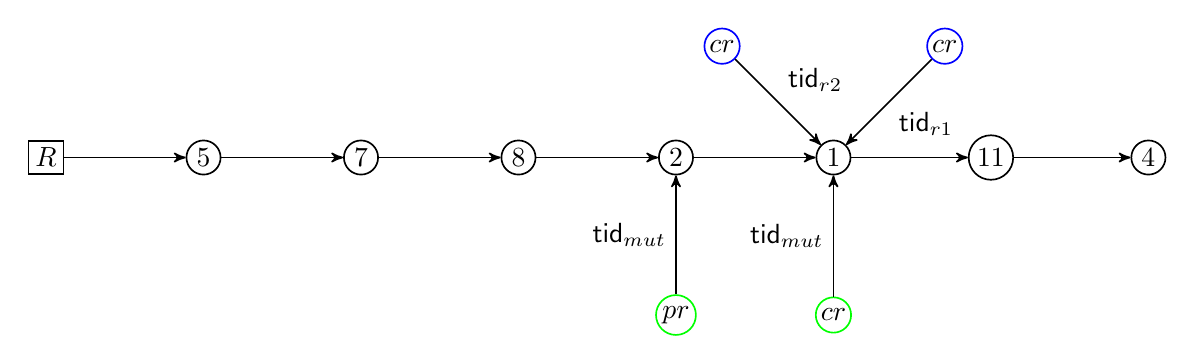
\begin{tikzpicture}[>=stealth',node distance=2cm,semithick,auto]
\tikzstyle{hollow node}=[circle,draw,inner sep=1.5]
\tikzstyle{sub node}=[triangle,draw,inner sep=1.5]
\tikzstyle{solid node}=[rectangle,draw,inner sep=2.5]

\tikzset{
	red node/.style={rectangle,draw=red,fill=red,inner sep=2.2},
	blue node/.style={rectangle,draw=blue,inner sep=2.5},
	reader node/.style={circle,draw=blue,inner sep=1},
	writer node/.style={circle,draw=green,inner sep=1}
}
 
      \node[solid node] (R) {$R$};
      \node[hollow node] (5) [right of=R] {$5$};
      \node[hollow node] (7) [right of=5] {$7$};
      \node[hollow node] (8) [right of=7] {$8$};
      \node[hollow node] (2) [right of=8] {$2$};
      \node[hollow node] (1) [right of=2] {$1$};
      \node[hollow node] (11) [right of=1] {$11$};
      \node[hollow node] (4) [right of=11] {$4$};
      \node[reader node] (r1) [above right of= 1]  {$cr$};
      \node[reader node] (r2)  [above left of= 1] {$cr$};
      \node[writer node] (wp) [below of=2] {$pr$}; 
      \node[writer node] (wc) [below of=1]{$cr$};

    \path[->]   (R) edge node {} (5)
                (5) edge node {} (7)
    		(7) edge node {} (8)
     		(8) edge node {} (2)
     		(11) edge node {} (4)   	
    		(1) edge node {} (11)
		(2) edge node {} (1)	
		(r1) edge node {$\textsf{tid}_{r1}$} (1)
		(r2) edge node {$\textsf{tid}_{r2}$} (1)
	        (wp) edge node  {$\textsf{tid}_{mut}$}  (2) 
		(wc) edge  node  {$\textsf{tid}_{mut}$}   (1)    
;
\end{tikzpicture}
\caption{A mutator thread with $\textsf{tid}_{mut}$ id is on linked list, $ l = \textsf{tid}_{mut}$, to delete the node with value 1.  Mutator thread has two iterators which are green $\textsf{pr}$ for showing previous node and  $\textsf{cr}$ for current node. }
\label{fig:mutatelist}
\end{figure}

\begin{figure}
\centering
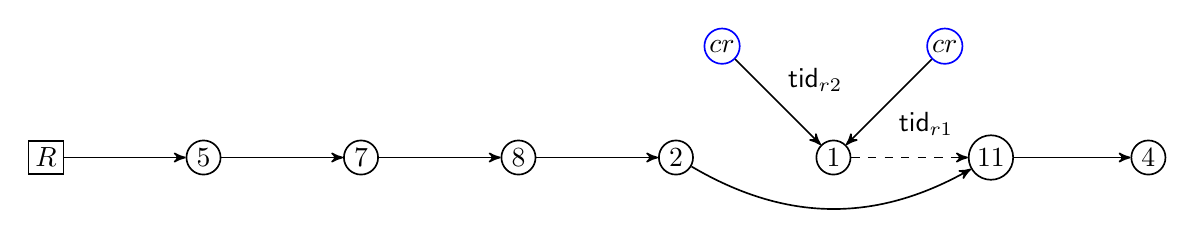
\begin{tikzpicture}[>=stealth',node distance=2cm,semithick,auto]
\tikzstyle{hollow node}=[circle,draw,inner sep=1.5]
\tikzstyle{sub node}=[triangle,draw,inner sep=1.5]
\tikzstyle{solid node}=[rectangle,draw,inner sep=2.5]

\tikzset{
	red node/.style={rectangle,draw=red,fill=red,inner sep=2.2},
	blue node/.style={rectangle,draw=blue,inner sep=2.5},
	reader node/.style={circle,draw=blue,inner sep=1},
	writer node/.style={circle,draw=green,inner sep=1}
}
 
      \node[solid node] (R) {$R$};
      \node[hollow node] (5) [right of=R] {$5$};
      \node[hollow node] (7) [right of=5] {$7$};
      \node[hollow node] (8) [right of=7] {$8$};
      \node[hollow node] (2) [right of=8] {$2$};
      \node[hollow node] (1) [right of=2] {$1$};
      \node[hollow node] (11) [right of=1] {$11$};
      \node[hollow node] (4) [right of=11] {$4$};
      \node[reader node] (r1) [above right of= 1]  {$cr$};
      \node[reader node] (r2)  [above left of= 1] {$cr$};


    \path[->]  (R) edge node {} (5);
    \path[->]  (5) edge node {} (7);
    \path[->]  (7) edge node {} (8);
    \path[->]  (8) edge node {} (2);
    \path[->]  (11) edge node {} (4);   	
    \path[->] (2) edge [bend right] node {} (11);
    \path[dashed,->]  (1) edge node {} (11);
   
    \path[->]  (r1) edge node {$\textsf{tid}_{r1}$} (1);
    \path[->]  (r2) edge node {$\textsf{tid}_{r2}$} (1);
;
\end{tikzpicture}

\caption{Linked-List is in a state where mutator thread with $\textsf{tid}_{mut}$ id unlinked the node with value 1 and released  $\textsf{pr}$ and $\textsf{cr}$ pointers on linked list, exited $\textsf{rcuMutate}$, $l \neq \textsf{tid}_{mut}$ . A unique thread for garbage collection, $\textsf{tid}_{gc}$, shows grace until all readers exit $\textsf{rcuRead}$.  Assuming that  location of the node with value 1 is $o$ then ($\textsf{tid}_{r2}$ ,o) $\in$ $F$ and ($\textsf{tid}_{r2}$,o) $\in$ $F$ }
\label{fig:unlinkedlist}
\end{figure}
RCU and similar programming patterns have an optimistic memory access pattern which stems from allowing access to memory locations while they are being updated by concurrent threads.  The crucial point on memory management to provide safe memory is deciding when to reclaim memory; e.g., deciding when it is safe to reclaim a node with value $1$ as in Figure ~\ref{fig:unlinkedlist}. RCU orchestrates threads reading, mutating and reclaiming a memory location in a data structure by letting a memory reclaimer wait for all reader threads to finish their $\textsf{rcuRead}$ sections before allocating the node.

Eventhough the protocols orchestrating threads in the RCU pattern can be expressed clearly in a few sentences, their implementations in non-blocking data structures are extremely subtle.  For example, in the non-blocking linked list implementation in Table ~\ref{tab:rculist}  unlinking a node in $\textsf{rcuMutate}$ involves more than a simple pointer setting. We can conclude that such an optimistic memory access pattern generates structures for which it is hard to reason for memory safety and other properties. We propose a $\textsf{Flow Sensitive}$ type system using $\textsf{Ownership Types}$ which enforces correct usage of RCU pattern  and comes with strong guarantees like $\textsf{Memory Safety}$ and some $\textsf{Linearisability}$ properties. 

\paragraph{Flow Sensitive} Our type system is flow sensitive, which means types of memory locations can be viewed [TODO: I do not like "view", find another] as different types under the permission of typing rules. For example, type $\textsf{undef}$ represents variables that can not be accessed until something is loaded into them. This is used in the flow sensitive type system to invalidate variables that should no longer be accessed. Another example is for the type, $\textsf{rcuIterator}$, which represents a pointer into an RCU data structure that can be used in either a $\textsf{rcuUpdate}$ or a $\textsf{rcuRead}$.
\paragraph{Ownership Types} A memory region can be observed either $\textsf{unlinked}$, $\textsf{fresh}$ or being accessed by a thread with an iterator on it , $\textsf{iterator tid}$.  If a memory region is observed as a part of RCU structure which means has field type $\textsf{rcu}$ then it is a unique part of $\textsf{rcu}$ typed structure or is $\textsf{unlinked}$  or is in the free list. More formal $\textbf{\textsf{Ownership}}$ definition is in section ~\ref{subsec:meminv} 
\paragraph{Linearisability} The fundemantal mechanism to guarantee some $\textsf{Linearisability}$ properties is providing $\textsf{linearity}$ for $\textsf{rcuIterator}$ of reader thread.  In other words, there is at most one $\textsf{rcuIterator}$ type for a thread for providing a reader thread not to read the same state more than once.  $\textbf{\textsf{Read Block Axioms}}$ in section ~\ref{readblockaxioms} has more rigorous definition of providing $\textsf{linearity}$. For the RCU-based Linked-List example, a generic $\textsf{Linearisability}$ condition that our type system provides is the condition for setting a value in the reader that can be satisfied by at most one node in the list.
\paragraph{Memory Safety} 

\end{document}
